\documentclass{article}
\usepackage[toc,page]{appendix}

\usepackage[preprint]{neurips_2023}
\usepackage[utf8]{inputenc} % allow utf-8 input
\usepackage[T1]{fontenc}    % use 8-bit T1 fonts
\usepackage{hyperref}       % hyperlinks
\usepackage{url}            % simple URL typesetting
\usepackage{booktabs}       % professional-quality tables
\usepackage{amsfonts}       % blackboard math symbols
\usepackage{nicefrac}       % compact symbols for 1/2, etc.
\usepackage{microtype}      % microtypography
\usepackage{xcolor}         % colors
\usepackage{hyperref}       % links

\usepackage{graphicx}       % include graphics
\usepackage{float}
\usepackage[T1]{fontenc}

\usepackage{caption}
\usepackage{subcaption}

\usepackage{multirow}

\newcommand{\sais}{Scottish Avalanche Information Service}
\newcommand{\usfs}{US Forest Service National Avalanche Center}

\title{ 	}


\author{
  Witold Gawlikowicz \\
  \texttt{witold@stanford.edu}
}


\begin{document}

\maketitle

\graphicspath{{assets/figures/}}


% \begin{abstract}
% \end{abstract}



\section{Introduction}

	Every year around a 100 people loose their lives to avalanches \href{https://www.avalanches.org/fatalities/}{in Europe alone} despite the fact that avalanche danger level forecasts are widely available there. There are many mountainous regions around the world for which no such forecasts are published, therefore automating the process of avalanche forecast generation could have real impact on lives of many people around the world. \\

	The main part of the avalanche danger level forecast for a given region is the overall avalanche danger level. It's expressed on a 5 point scale ranging from 1 (lowest) to 5 (highest).	\href{https://www.shastaavalanche.org/page/how-read-advisory}{Forecasts} for many regions often also contain: \href{https://avalanche.state.co.us/forecasts/tutorial/avalanche-problems}{the avalanche problems} (main characteristics of the snowpack which contribute to its instability and hence potential avalanche), the aspect-elevation rose which shows more fine-grained avalanche danger levels broken down by slope's aspect and elevation and a descriptive part discussing conditions and how they might change during the day in more detail. \\
	The primary goal of this project is to use the overall avalanche danger level forecast for the region as the dependent variable and see to what extent it can be modelled with weather data.
	
\section{Data}

	% This section briefly describes the datasets collected to date.

\subsection{\sais}\label{sec:data_sais}

	The \href{https://www.sais.gov.uk/forecast-archive/}{Scottish Avalanche Information Service} (SAIS) provides historical avalanche forecasts for 6 regions in Scotland. The forecasts are typically published from December to April. SAIS allows bulk download of snowprofile data containing avalanche hazard level as well as snowprofile data collected during compilation of observed hazard levels. The size of the dataset prior to any cleansing was \input{assets/snippets/sais_size_initial.txt}observations.
	\newline
	The dataset contains two variables either of which could be used as our dependent variable: observed and forecasted avalanche hazard level.
	The forecasted value is decided on by avalanche professionals working in a given area based on the current state of the snowpack and the weather forecast for the next day.
	The observed value (nowcast) is updated on the day.
	\newline
	While both values are compiled using a standardised methodology, there is an inherent subjectivity in both of them, but especially so in the nowcast as it relies a lot on travel throughout the area and multifaceted, in-person assessment of the snow conditions. For that reason we will use the forecasted value as our dependent variable as it should be more standardised, have a clearer relationship with the weather inputs, and thus it should be more feasible for the model to discover the underlying relationship between the variables.

\subsubsection{Data transformations}
	Since the hazard level "5" doesn't feature in our dataset we consider only hazard levels 1-4. Level "5" is very rare for most avalanche centres, and in most avalanche scales the difference between levels "4" and "5" doens't relate to the hazard intensity, but potential for destruction of infrastrcture (clearly not the case in all avalanche regions as some of them are quite remote). It is common practice when modelling avalanche hazard levels to merge those two levels together. 
	We have dropped missing values of both potential independent variables and used various strategies (details in \href{https://github.com/witgaw/avalanche-danger-level-forecast/blob/project-report/src/data-exploration-hazard-levels.ipynb}{\texttt{data-exploration-hazard-levels.ipynb}}) for filling missing data brining the number of observations down to \input{assets/snippets/sais_size_final.txt}\unskip.\\
	\newline 
	We set aside 20\% of the data as the test set stratifying on avalanche hazard levels. We have decided not to use a development set and rely on cross-validation instead.
	% \begin{table}[H]
\centering
\caption{\detokenize{"mapped_hazard_forecast"} per dataset split}
\label{tbl:sais_hazard_breakdown_per_split}
\begin{tabular}{rrrr}
\toprule
\detokenize{mapped hazard forecast} & Train & Dev & Test \\
\midrule
1 & 2073 & 518 & 545 \\
2 & 2070 & 517 & 405 \\
3 & 2476 & 620 & 131 \\
4 & 380 & 95 & 1 \\
\bottomrule
\end{tabular}
\end{table}


\subsection{Weather data}
While \href{https://meteostat.net}{open source data} providers exist, to the best of our knowledge these only provide data from specific weather stations. Proprietary data providers often also offer data interpolated to a specific location using a weather model, hence we decided to use that kind of that for this project. Unfortunately, at the time of writing permission to open source this data has not been obtained hence it remains in a seprate private repository added to the main project repository as a submodule. The author is happy to help facilitate access to it for grading purposes if needed and for interested researchers.

The weather data for the highest summit in each of the 6 forecast zones has been downloaded from \href{https://www.visualcrossing.com/}{Visual Crossing}.  All the standard atmospheric variables like temperature, humidity, precipitation, wind speed and direction have been downloaded. Additionally, selected \href{https://www.visualcrossing.com/resources/documentation/weather-api/agriculture-elements-in-the-timeline-weather-api/}{agricultural} and \href{https://www.visualcrossing.com/resources/documentation/weather-api/energy-elements-in-the-timeline-weather-api/}{energy} data points have been downloaded. Details can be found in \href{https://github.com/witgaw/avalanche-danger-level-forecast/blob/project-report/src/data-exploration-weather.ipynb}{\texttt{data-exploration-weather.ipynb}}.
	Data has been downloaded for all the dates for which SAIS hazard levels were available. Data has been downloaded in both daily and hourly resolution. 
	While the API allowed download of both observed and historically forecasted value we have opted only for the observed values as historical forecasts were not available prior to 2020 for the selected locations. Since our data set spanned dates from 2007 to 2024 limiting our dataset to only the dates for which historical forecasts were available would significantly reduce its size. Mixing observed and forecasted variables in the same columns would potentially negatively impact models' performance. However, it should be noted that ideally we would like to use observed data for all the days prior to the date for which the forecast is being generated and a historical day-ahead forecast for the that date. Therefore it should be noted that the actual performance of the model might differ depending on the quality of the forecast.

\subsubsection{Data transformations}\label{sec:weather_data_trans}
	Since avalanches, and thus avalanche hazard forecasts, are impacted by weather not just the day before the warning is issued but over many days prior, or even the entire season, we have transformed the data so that our independent variables reflect that. For the day for which the hazard level is modelled, as well as the day prior,u we use hourly data for all the variables considered. For all previous days we use daily data. We account for \input{assets/snippets/sais_avg_season_length.txt}days as that's the average season length in our dataset. All the entires prior to season's begining are set to 0. Thus the vectors are sparser the closer to the begining of the season the modelled hazard level is. After cleaning up the data to remove missing variables the dimensionality of the independent variable vector is \input{assets/snippets/weather_idependent_variable_dimension.txt}\unskip.

\section{Model fitting}

	In this section, we describe the process of fitting machine learning models to the collected data. We fit each model using the default parameters provided by the \texttt{scikit-learn} library and then carry out hyperparameter optimisation of selected paramters using 10-fold cross-validation repeated 3 times to reduce the noise in model performance estimate. We use a random parameter space search with 20 iterations. We use the macro-averaged $F_1$ score as the metric used for parameter tuning. Details can be found in \href{https://github.com/witgaw/avalanche-danger-level-forecast/blob/project-report/src/modelling.ipynb}{\texttt{modelling.ipynb}}.
	For all models we use dependent variables described in Section \ref{sec:weather_data_trans}.
	All of the models are used as classifiers outputting one of the 4 avalanche hazard levels considered.

\subsection{Softmax regression}

	Softmax regression, also known as multinomial logistic regression, is a generalization of logistic regression to multiple classes. It is a simple and interpretable model that serves as a good starting point. \\
	We have also run this model using the snow profiles dug on the day for which the forecast was made. While this is not how we envisage the model being run, as we would like to develop a flexible methodology that could eventually be used to model avalanche hazards in remote areas, it serves as a useful comparison in performance of model using specialised data gathered by domain-experts and generally available weather variables.

	Parameters considered during the hyperparameter optimisation step: solver, tolerance for stopping criteria, type of regularisation term, regularisation strength, whether an intercept term should be fitted or not, and weights assigned to each of the classes.

\subsection{Random forest}
	Due to promissing results of \cite{nhess-22-2031-2022} using random forest for dry-snow conditions in Switzerland we have decided to see how this model will perform on our dataset. Random forest is an ensemble learning technique combining multiple decision trees and averaging their results to generate the output which helps to reduce the tendency of decision trees to overfit the data.

	Parameters considered during the hyperparameter optimisation step: number of random trees, the function to measure quality of a split, the maximum number of features to consider when generating a split, maximum depth of a tree and weights assigned to each of the classes.

\subsection{Multi-layer perceptron (MLP)}
	While \texttt{scikit-learn} is not a dedicated Deep learning library it does contain an implementation of a multi-layer perceptron. Due to the high dimensionality of the data, highly non-linear relationship between weather data across the entire seasons and avalanche level, and since we are dealing with a classification problem, a multi-layer neural network seemed like a promissing approach to try out for our problem.

	Parameters considered during the hyperparameter optimisation step: solver type, the size and number of hidden layers, activation function, momentum for gradient descent update within the Adam optimiser, the strength of L2 regularisation term and the learning rate.

\section{Evaluation}\label{sec:evaluation}

The metrics which we evaluate for each model include: accuracy, precision, recall and $F_1$ score. Precision, recall and $F_1$ score are computed per-class, as well as macro-averaged.
\newline
We have also included the mean squared errors computed on mapped classes (integers from 1 to 4) and average error ($y^{true} - y^{predicted}$). The last metric is constructed to give a basic understanding of model's under- or over-reporting of the hazard level.

\subsection{Baseline fits}

To get a better feel for how the different metrics are behaving on this dataset we will compute two baselines: 
\begin{enumerate}
	\item A constant model that always predicts the most common class in the training set (hazard level "3").
	\item "Observed" model returning the observed avalanche hazard level discussed in Section \ref{sec:data_sais}.
\end{enumerate}
The idea is that the first baseline will provide a lower bound on the performance of any model we might want to begin to consider and the second one will likely be the upper bound as it's compiled by the same experts who made the forecast, but with the additional benefit of being able to directly observe the actual changes in the snowpack.

Metrics for those baselines and all the models considered will be included in Section \ref{sec:evaluation}.

	The evaluation metrics for each model computed on the test set are presented in Table \ref{tbl:sais_eval_test} below. 


	\begin{table}[H]
\caption{Evaluation metrics computed on the test set}
\label{tbl:sais_eval_test}
\begin{tabular}{lllll}
\toprule
 & constant & observed & softmax regression (snow profiles) & softmax regression (snow profiles tabularised) \\
\midrule
MSE & 2.4 & 0.2 & 0.3 & 1.9 \\
average error & -1.4 & 0.1 & 0.0 & -0.7 \\
highest error & -2 & 2 & 2 & -3 \\
accuracy & 0.1 & 0.8 & 0.7 & 0.3 \\
precision (multiclass) & [0.0, 0.0, 0.12, 0.0] & [0.82, 0.78, 0.89, 0.0] & [0.79, 0.65, 0.43, 0.0] & [0.55, 0.39, 0.13, 0.01] \\
precision (micro) & 0.1 & 0.8 & 0.7 & 0.3 \\
precision (macro) & 0.0 & 0.6 & 0.5 & 0.3 \\
recall (multiclass) & [0.0, 0.0, 1.0, 0.0] & [0.93, 0.71, 0.63, 0.0] & [0.88, 0.46, 0.63, 0.0] & [0.3, 0.25, 0.39, 1.0] \\
recall (micro) & 0.1 & 0.8 & 0.7 & 0.3 \\
recall (macro) & 0.2 & 0.6 & 0.5 & 0.5 \\
$F_1$ (multiclass) & [0.0, 0.0, 0.22, 0.0] & [0.87, 0.74, 0.74, 0.0] & [0.84, 0.54, 0.51, 0.0] & [0.39, 0.31, 0.2, 0.01] \\
$F_1$ (micro) & 0.1 & 0.8 & 0.7 & 0.3 \\
$F_1$ (macro) & 0.1 & 0.6 & 0.5 & 0.2 \\
\bottomrule
\end{tabular}
\end{table}


	\begin{figure}[h]
		\centering
		\begin{subfigure}[b]{0.49\textwidth}
			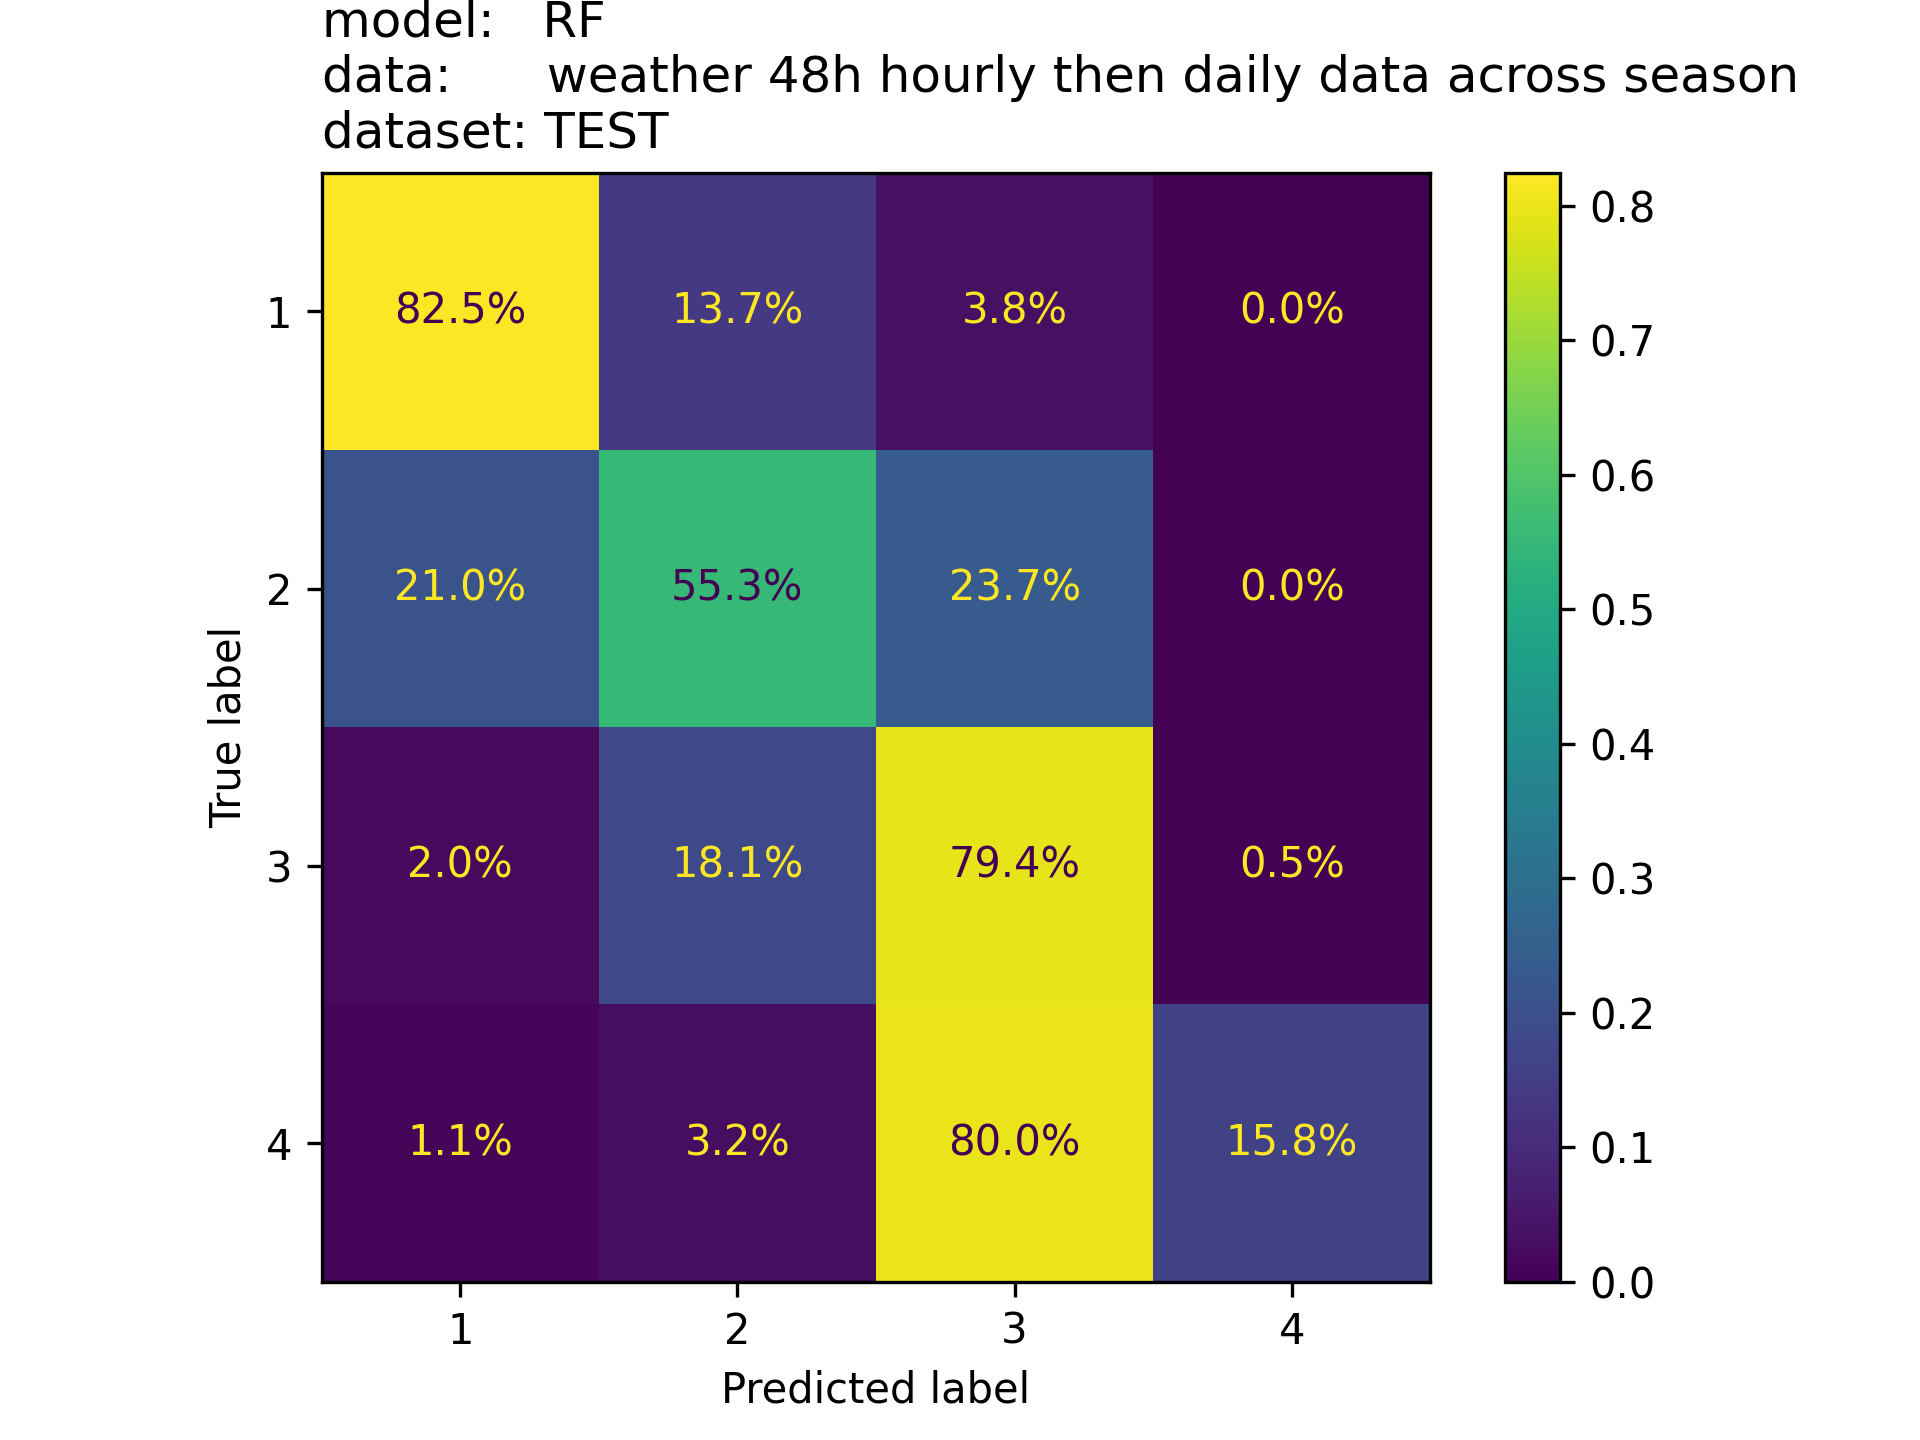
\includegraphics[width=\textwidth]{sais_confusion_matrix_RF_____weather_48h_hourly_then_daily_data_across_season_test.png}
			\caption{Default parameters.}
		\end{subfigure}
		\hfill
		\begin{subfigure}[b]{0.49\textwidth}
			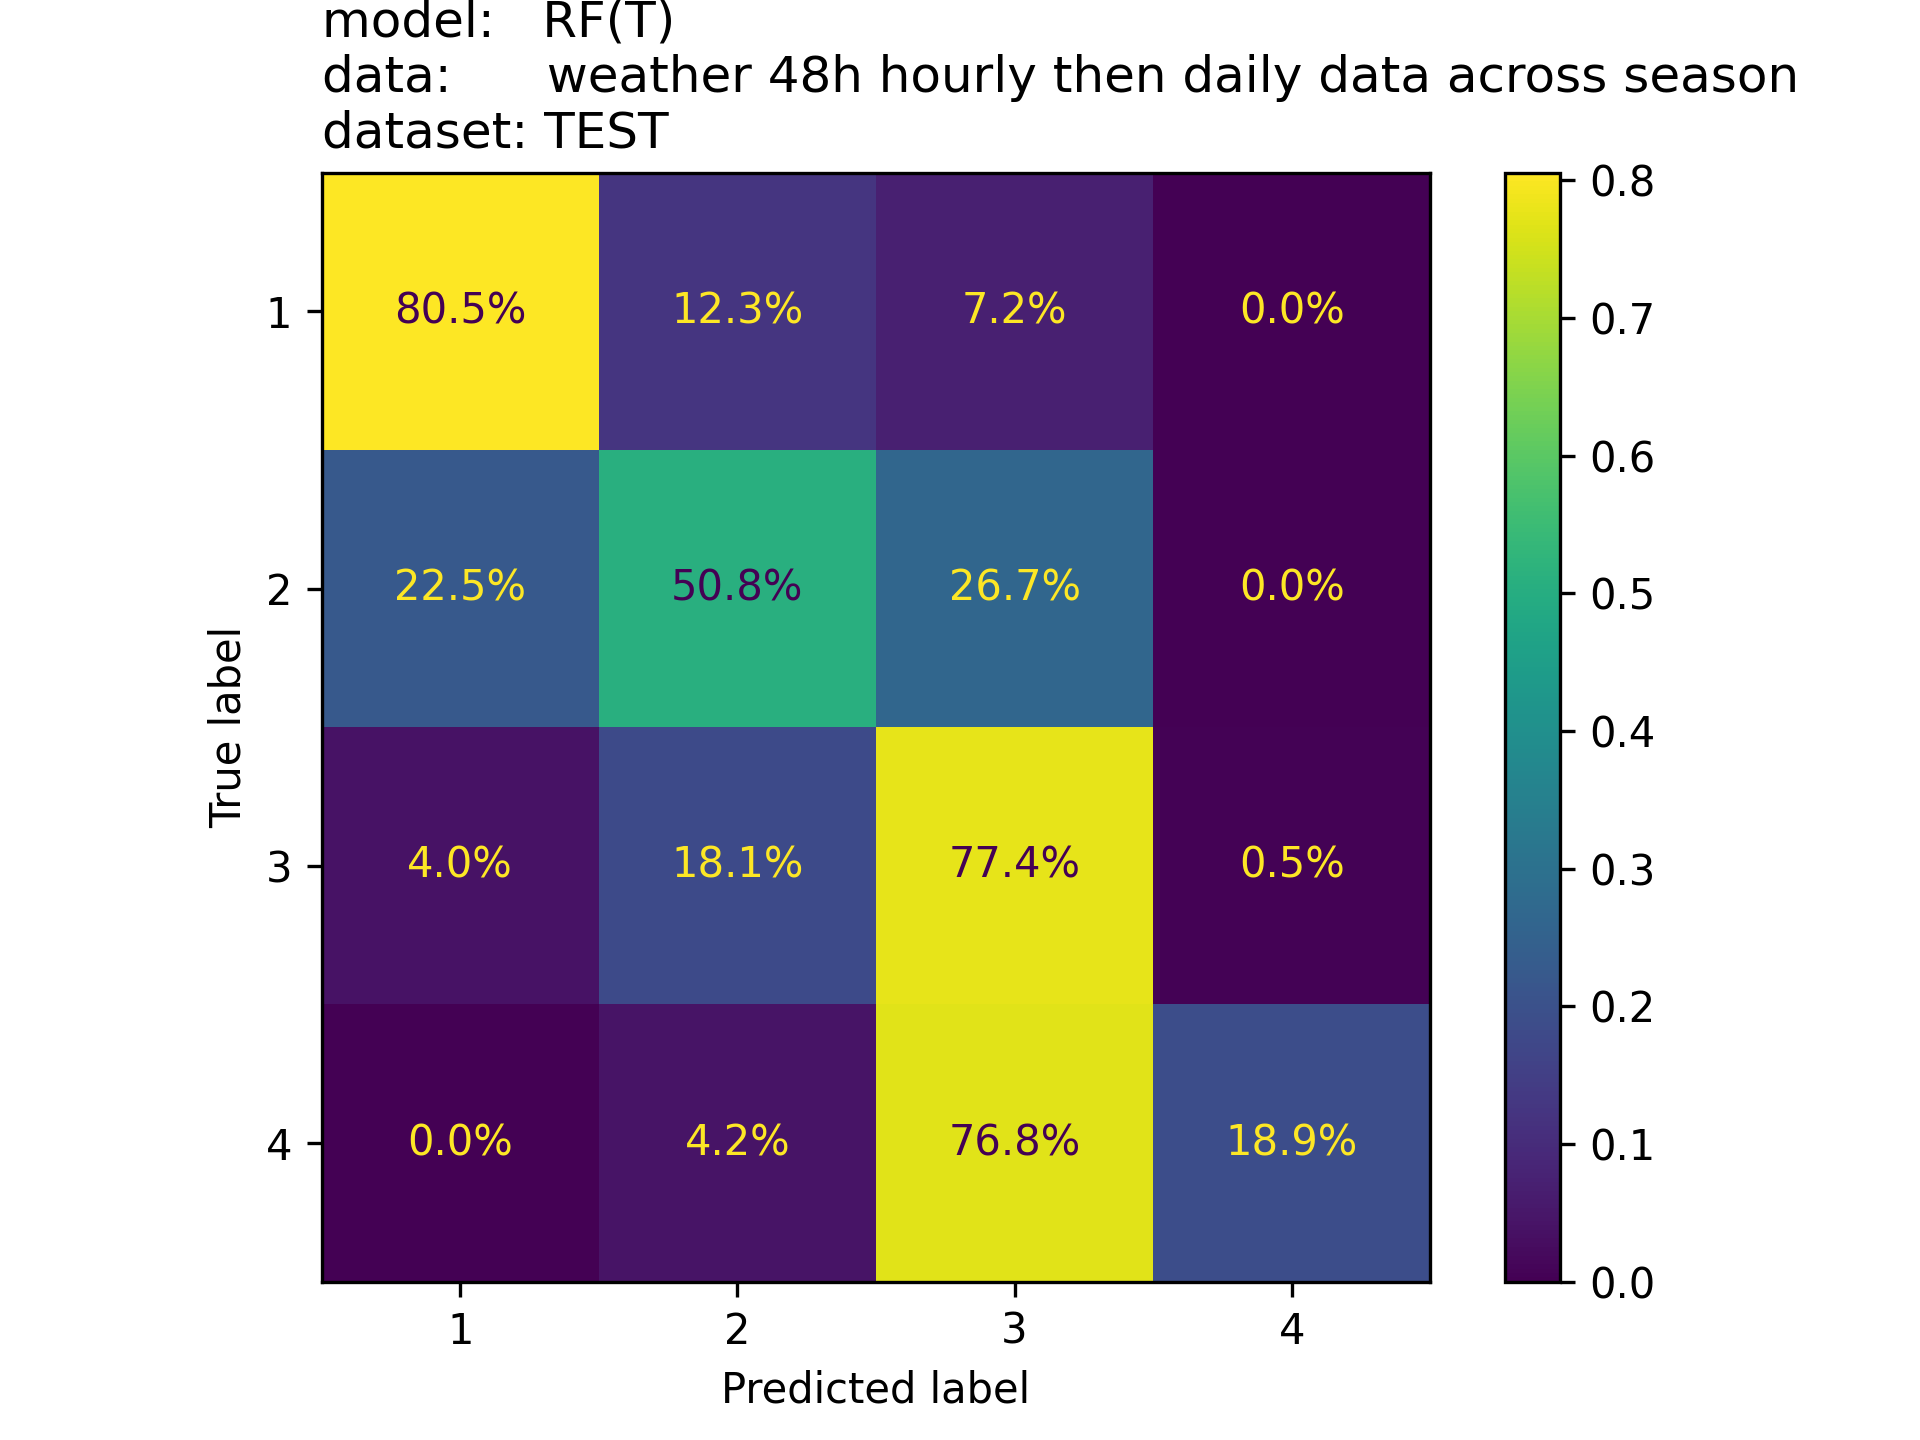
\includegraphics[width=\textwidth]{sais_confusion_matrix_RF(T)__weather_48h_hourly_then_daily_data_across_season_test.png}
			\caption{Optimised hyperparameters}

		\end{subfigure}
		\caption{Random forest on Test set.}
		\label{fig:rf}
	\end{figure}

	\begin{figure}[h]
		\centering
		\begin{subfigure}[b]{0.49\textwidth}
			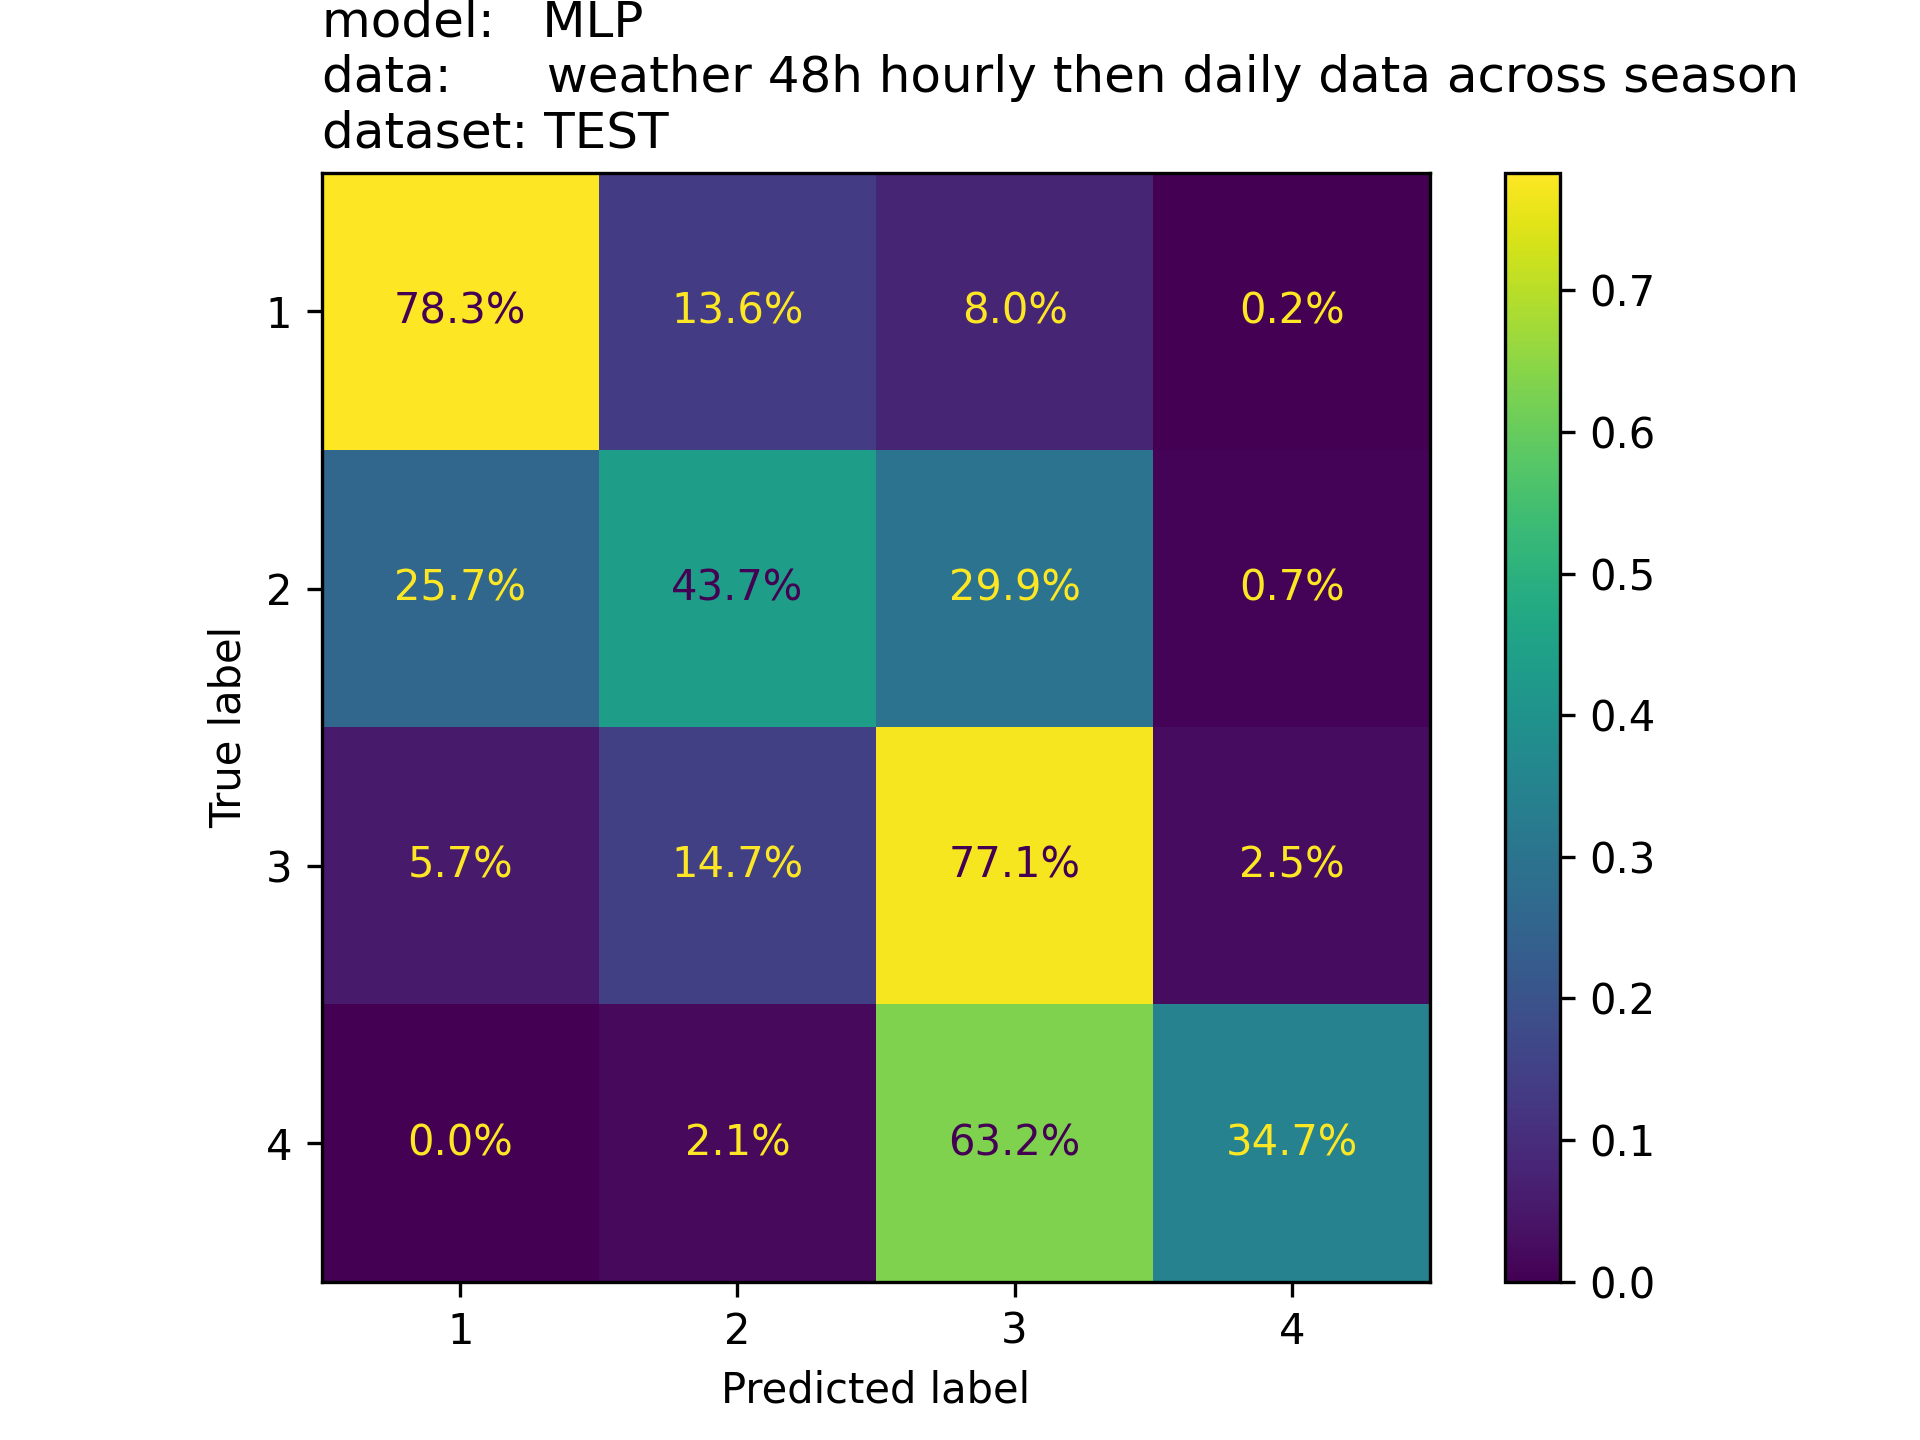
\includegraphics[width=\textwidth]{sais_confusion_matrix_MLP____weather_48h_hourly_then_daily_data_across_season_test.png}
			\caption{Default parameters.}
		\end{subfigure}
		\hfill
		\begin{subfigure}[b]{0.49\textwidth}
			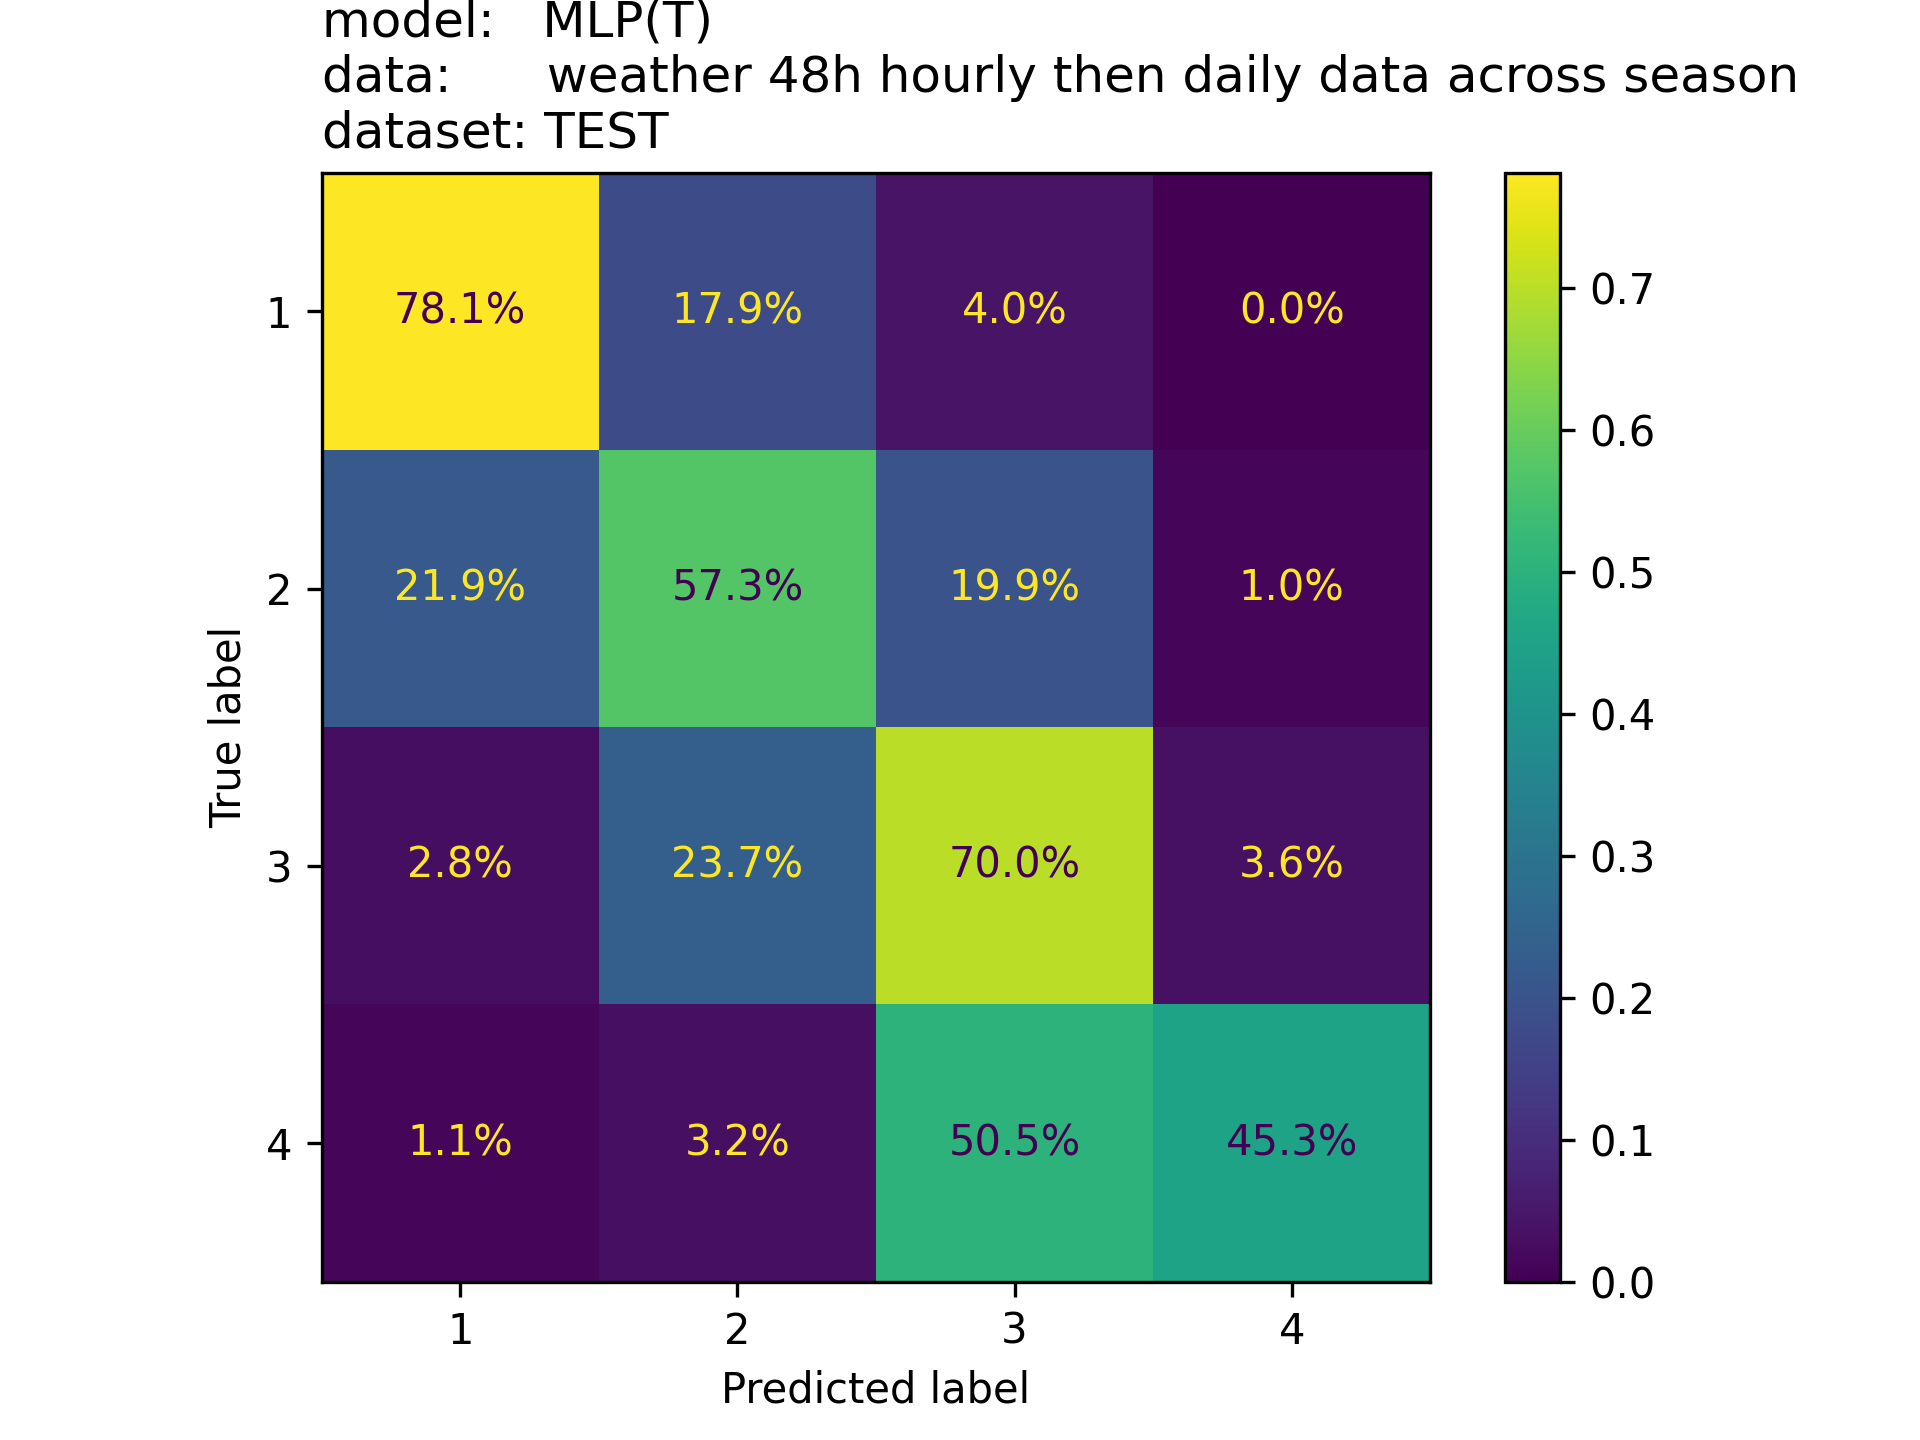
\includegraphics[width=\textwidth]{sais_confusion_matrix_MLP(T)_weather_48h_hourly_then_daily_data_across_season_test.png}
			\caption{Optimised hyperparameters}
		\end{subfigure}
		\caption{Multi-layer perceptron on Test set.}
		\label{fig:mlp}
	\end{figure}

\section{Conclusion and future work}
	As we can see in Figure \ref{fig:rf} the random forest classifier peforms quite well for labels 1-3, but fails badly as far as hazard level "4" is concenred, where majority of the datapoints from the test set get incorrectly classified as hazard level "3". Hyperparameter tuning only slightly improves this problem and it actually reduces performance for class "2".

	The multi-layer perceptron classifier (Figure \ref{fig:mlp}) is the most promising of the classifiers considered. The performance with default parameters for classes "2" and "4" is sub-par, however hyperparameter optimisation brings about significant improvements in that regard.
	In fact it's not as dissimilar to results presented in Figure 4 in \cite{egusphere-2024-2374} as one might expect. The mentioned figure shows performance of a random forest classifier used for avalanche danger level prediction in Swiss alps. As the paper mentions, this model has in fact been used operationally for several seasons now. It highlights similar issues to the ones observed in this project: while accurate prediction of hazard levels "1" and "3" is achievable, levels "2" and "4" are much more difficult to characterise accurately. \\

	Future work on this project will focus on reproducing the results obtained for the SAIS dataset on the US dataset obtained as part of this project. Since the results obtained with MLP were the most promissing, another avenue worth exploring seems to be moving to a more Deep learning oriented library like PyTorch or TensorFlow and exploring multilayer neural networks with more complex topologies, as well getting more compute resources employed (this project was done entirely on an M1 Mac).

	As mentioned in the introduction, avalanche reports contain much more information than just the avalanche hazard levels. Incorporating terrain features (\cite{egusphere-2023-2948}) to allow for generation of the aspect-elevation rose as well as better generalisation of the model to areas it has not been trained on will be one of the future goals for this project. Lastly, we would like to explore the possibility of predicting the avalanche problem (\cite{MORIN2020102910} \cite{REUTER2022103462}) from data.

	\section*{Acknowledgements}
	I would like to express my deepest gratitude to all the people and entities who helped me during my work on this project:\\
			% \begin{itemize}
			\newline
			\textbf{Chris Lundy}, National Avalanche Specialist from USDA Forest Service National Avalanche Center, for providing me with access to the historical danger level forecasts from all the avalanche centres across US and allowing me to open-source the dataset, as well as for professionally and patiently answering my numerous questions. \\
			\textbf{Mark Diggins}, Co-ordinator for Scottish Avalanche Information Service, for helping me to swiftly and easily download the historical avalanche danger level for Scotland which formed the main focus of this project.\\
			\textbf{Boxin Zhang} for project mentorship.\\
			\href{https://www.visualcrossing.com/}{Visual Crossing} for granting me access to their proprietary historical weather data API with a generous calls quota free of charge for research purposes as well as providing me with timely and professional support.\\
			\href{https://www.meteoblue.com/}{Meteoblue} for granting me access to their proprietary historical weather data API for 3 locations as well as a quota of general API calls free of charge.\\
			\href{https://github.com/}{GitHub} for their free Student Developer Pack including Copilot which has been used for generating isolated code snippets used in this project, mostly around Pandas DataFrame manipulation, function documentation and skeleton PyTest code generation.
			% \end{itemize}

\newpage
% \begin{appendices}
% 	\newpage
% 	\section{Dataset details}
% 	This section contains further details of the datasets used for the project.

% 	% \begin{table}[H]
\caption{Summary of the SAIS dataset prior to any modifications}
\label{tbl:sais_summary_initial}
\begin{tabular}{rrllll}
\toprule
non-null & unique & dtype & mean & min & max \\
\midrule
17453 & 12045 & datetime64[ns] & 2011-03-06 & 1993-12-20 & 2024-04-13 \\
17453 & 6 & object & NaN & NaN & NaN \\
11402 & 791 & object & NaN & NaN & NaN \\
11291 & 3557 & object & NaN & NaN & NaN \\
17434 & 683 & object & NaN & NaN & NaN \\
17095 & 337 & float64 & 97.1 & -1.0 & 163770.0 \\
17384 & 56 & float64 & 17.8 & -1.0 & 1020.0 \\
11409 & 3497 & object & NaN & NaN & NaN \\
17389 & 520 & object & NaN & NaN & NaN \\
17221 & 366 & float64 & 199.0 & -9999.0 & 905.0 \\
17376 & 107 & float64 & 14.2 & -9999.0 & 360.0 \\
17402 & 38 & float64 & 73.3 & -9999.0 & 199.0 \\
10756 & 9 & object & NaN & NaN & NaN \\
17452 & 6 & object & NaN & NaN & NaN \\
17194 & 279 & float64 & 65.3 & -1.0 & 3000.0 \\
17380 & 87 & float64 & 1.0 & -9999.0 & 310.0 \\
14028 & 28 & float64 & 0.4 & -1.0 & 55.0 \\
17453 & 3 & int64 & -11.3 & -9999.0 & 1.0 \\
16253 & 222 & float64 & -0.8 & -13.4 & 15.0 \\
15638 & 357 & float64 & 123.4 & -2.0 & 2213.0 \\
16039 & 153 & float64 & 17.7 & -8.0 & 360.0 \\
11310 & 6 & object & NaN & NaN & NaN \\
11792 & 6 & object & NaN & NaN & NaN \\
17090 & 214 & object & NaN & NaN & NaN \\
16811 & 120 & float64 & 1.2 & 0.0 & 130.0 \\
16886 & 8 & float64 & 1.3 & 0.0 & 5.0 \\
16714 & 368 & float64 & 149.8 & -9999.0 & 676.0 \\
16234 & 58 & float64 & -3.8 & -9999.0 & 368.0 \\
16480 & 22 & float64 & -1.4 & -9999.0 & 208.0 \\
15988 & 11 & float64 & -6.8 & -9999.0 & 20.0 \\
16401 & 11 & float64 & -3.9 & -9999.0 & 10.0 \\
14457 & 20 & float64 & -3071.0 & -9999.0 & 8800.0 \\
16574 & 284 & float64 & -6.1 & -9999.0 & 125.0 \\
13736 & 5917 & object & NaN & NaN & NaN \\
\bottomrule
\end{tabular}
\end{table}

% 	\begin{figure}[h]
% 		\centering
% 		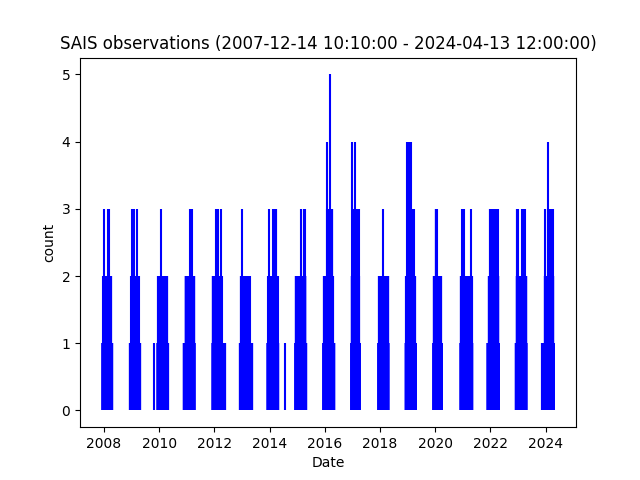
\includegraphics[width=0.7\textwidth]{sais_observation_histogram.png}
% 		\caption{Histogram of avalanche danger levels in the SAIS dataset.}
% 		\label{fig:sais_observation_histogram}
% 	\end{figure}

% 	\begin{table}[h]
\caption{Count of hazard levels and date ranges per area after dropping missing hazard values.}
\label{tbl:sais_area_breakdown}
\begin{tabular}{lrll}
\toprule
 & total & min date & max date \\
Area &  &  &  \\
\midrule
Creag Meagaidh & 1973 & 2007-12-21 & 2024-04-13 \\
Glencoe & 1991 & 2007-12-21 & 2024-04-13 \\
Lochaber & 2092 & 2007-12-14 & 2024-04-13 \\
Northern Cairngorms & 2125 & 2007-12-14 & 2024-04-13 \\
Southern Cairngorms & 1994 & 2007-12-21 & 2024-04-13 \\
Torridon & 1108 & 2013-12-24 & 2024-04-13 \\
\bottomrule
\end{tabular}
\end{table}

% 	\begin{table}[h]
\caption{\detokenize{"mapped_hazard_forecast"} breakdown per area}
\label{tbl:sais_mapped_hazard_breakdown_per_area}
\begin{tabular}{lrrrr}
\toprule
 & 1 & 2 & 3 & 4 \\
Area &  &  &  &  \\
\midrule
Creag Meagaidh & 462 & 609 & 777 & 125 \\
Glencoe & 559 & 558 & 735 & 139 \\
Lochaber & 544 & 561 & 840 & 147 \\
Northern Cairngorms & 546 & 639 & 829 & 111 \\
Southern Cairngorms & 662 & 590 & 646 & 96 \\
Torridon & 549 & 419 & 139 & 1 \\
\bottomrule
\end{tabular}
\end{table}

% 	% \begin{table}[h]
\caption{Training set: \detokenize{"mapped_hazard_forecast"} breakdown per area}
\label{tbl:sais_mapped_hazard_breakdown_per_area_train}
\begin{tabular}{lrrrr}
\toprule
 & 1 & 2 & 3 & 4 \\
Area &  &  &  &  \\
\midrule
Creag Meagaidh & 319 & 355 & 376 & 42 \\
Glencoe & 437 & 417 & 543 & 103 \\
Lochaber & 433 & 440 & 647 & 114 \\
Northern Cairngorms & 426 & 478 & 610 & 79 \\
Southern Cairngorms & 458 & 380 & 300 & 42 \\
\bottomrule
\end{tabular}
\end{table}

% 	% \begin{table}[H]
\caption{Summary of data cleansing actions on SAIS dataset}
\label{tbl:sais_replacements_log}
\begin{tabular}{ll}
\toprule
column name & action \\
\midrule
Forecast aval. hazard & 5661 missing values dropped \\
Observed aval. hazard & 509 missing values dropped \\
Air Temp & Change datatype to numeric \\
Drift & Change datatype to numeric \\
Summit Wind Dir & Set to 0 if "Summit Wind Speed" = 0 \\
Wind Dir & Set to 0 if "Wind Dir" = 0 \\
Summit Air Temp & Cross fill missing values with "Air Temp" \\
Summit Wind Dir & Cross fill missing values with "Wind Dir" \\
Summit Wind Speed & Cross fill missing values with "Wind Speed" \\
Precip Code & 605 NAs filled with "0 - None" \\
Foot Pen & 33 NAs filled with "0" \\
Ski Pen & 3356 NAs filled with "0" \\
Crystals & 1414 NAs filled with "0" \\
Wind Speed & 18 NAs filled with "0" \\
Summit Wind Speed & 18 NAs filled with "0" \\
Total Snow Depth & 221 NAs filled with "0" \\
Max Temp Grad & 557 NAs filled with "0" \\
Max Hardness Grad & 482 NAs filled with "0" \\
Snow Index & 1180 NAs filled with "0" \\
Wetness & 997 NAs filled with "0" \\
Precip Code & Split into "\detokenize{precip_code_numeric}" and "\detokenize{precip_code_desc}" \\
All columns & Drop 1049 with missing values \\
Wind Dir & Drop 15 negative values \\
Wind Speed & Drop 2 negative values \\
Cloud & Drop 1 negative values \\
Total Snow Depth & Drop 36 negative values \\
Foot Pen & Drop 2 negative values \\
Ski Pen & Drop 4 negative values \\
Summit Wind Dir & Drop 184 negative values \\
Summit Wind Speed & Drop 5 negative values \\
Snow Index & Drop 64 negative values \\
Insolation & Drop 2 negative values \\
Crystals & Drop 77 negative values \\
No Settle & Drop 4 negative values \\
Wetness & Drop 7 negative values \\
\bottomrule
\end{tabular}
\end{table}

% 	\newpage
% 	\section{Evaluation}
% 	\begin{figure}[h]
% 		\centering
% 			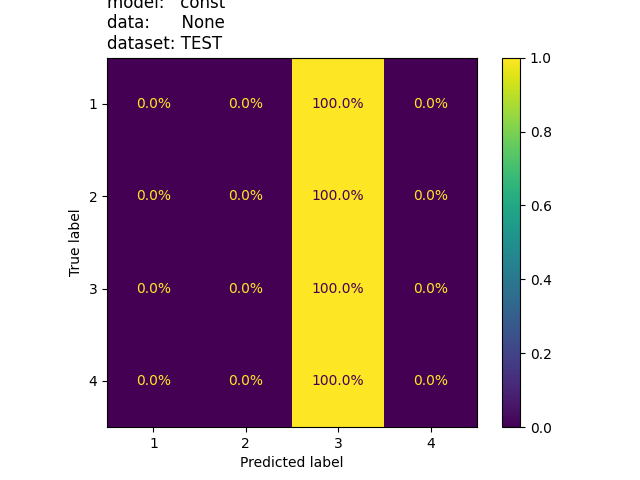
\includegraphics[width=\textwidth]{sais_confusion_matrix_const_None_test.png}
% 		\caption{Confusion matrix for constant model on test set.}
% 	\end{figure}

% 	\begin{figure}[h]
% 		\centering
% 		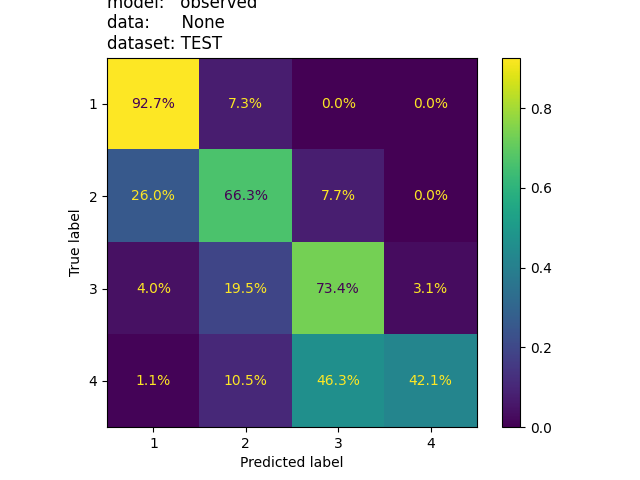
\includegraphics[width=\textwidth]{sais_confusion_matrix_observed_None_test.png}
% 		\caption{Confusion matrix for "observed" model on test set.}
% 	\end{figure}

% 	\begin{figure}[h]
% 		\centering
% 		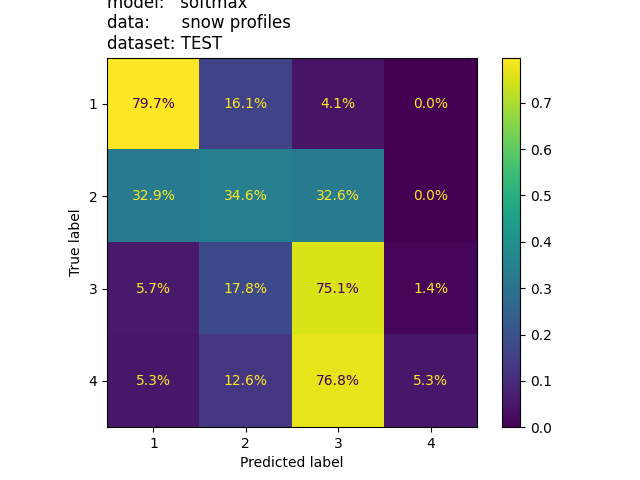
\includegraphics[width=\textwidth]{sais_confusion_matrix_softmax_snow_profiles_test.png}
% 		\caption{Confusion matrix for Softmax model on days' snowprofiles on test set.}
% 	\end{figure}

% \end{appendices}

\newpage
\bibliography{references}
\bibliographystyle{plainnat}

\end{document}

	% Leftovers:
	%	As the number of people participating in outdoor recreation is \href{https://americancanoe.org/wp-content/uploads/2023/06/2023_Outdoor_Participation_Trends_Report.pdf}{steadily growing in the US}, and likely most of the other countries with access to mountains too, a
	%	On a \href{https://avalanche.org/avalanche-encyclopedia/human/resources/north-american-public-avalanche-danger-scale/}{North American scale} the levels are: 1 - "low", 2 - "moderate", 3 - "considerable", 4 - "high", 5 - "extreme". 
	%	The \href{https://www.avalanches.org/standards/avalanche-danger-scale/}{European scale} is similar with level 5 being described as "very high". Due to the ongoing efforts of the global avalanche forecasting scientific community the forecasting terminology have been getting more standardised across the world. However, it has to be noted that regional difference may still be present. 
	%	aspect ("N", "NE", "E", "SE", "S", "SW", "W", "NW") and elevation (either absolute elevations applicable to a given region or relative elevations driven by tree cover: "below treeline", "near treeline", "above treeline").
